\documentclass{article}
\usepackage{graphicx} % Required for inserting images
\graphicspath{{./assets/}} % Specifies the directory where images are stored

\title{Assignment 3}
\author{Jacqueline Wu, Sam Zhang}
\date{March 2024}

\begin{document}

\maketitle

\section{Value-based method with linear function approximation}
We implement Q-Learning and Expected SARSA and experiment them with two environments from the Gymnasium, an open-source fork of the OpenAI Gym. \cite{gymnasium}
During the experiment, the environment's states are discretized through tile-coding into a binary vector.

\subsection{Results}
We experiment with 3 $\epsilon$ per algorithm-environment pair, and use a fixed set of 3 different learning rates $\alpha \in \{ \frac{1}{4}, \frac{1}{8}, \frac{1}{16} \}$. The results are shown in Figure \ref{fig:q1}.

\begin{figure}[htbp]
    \centering
    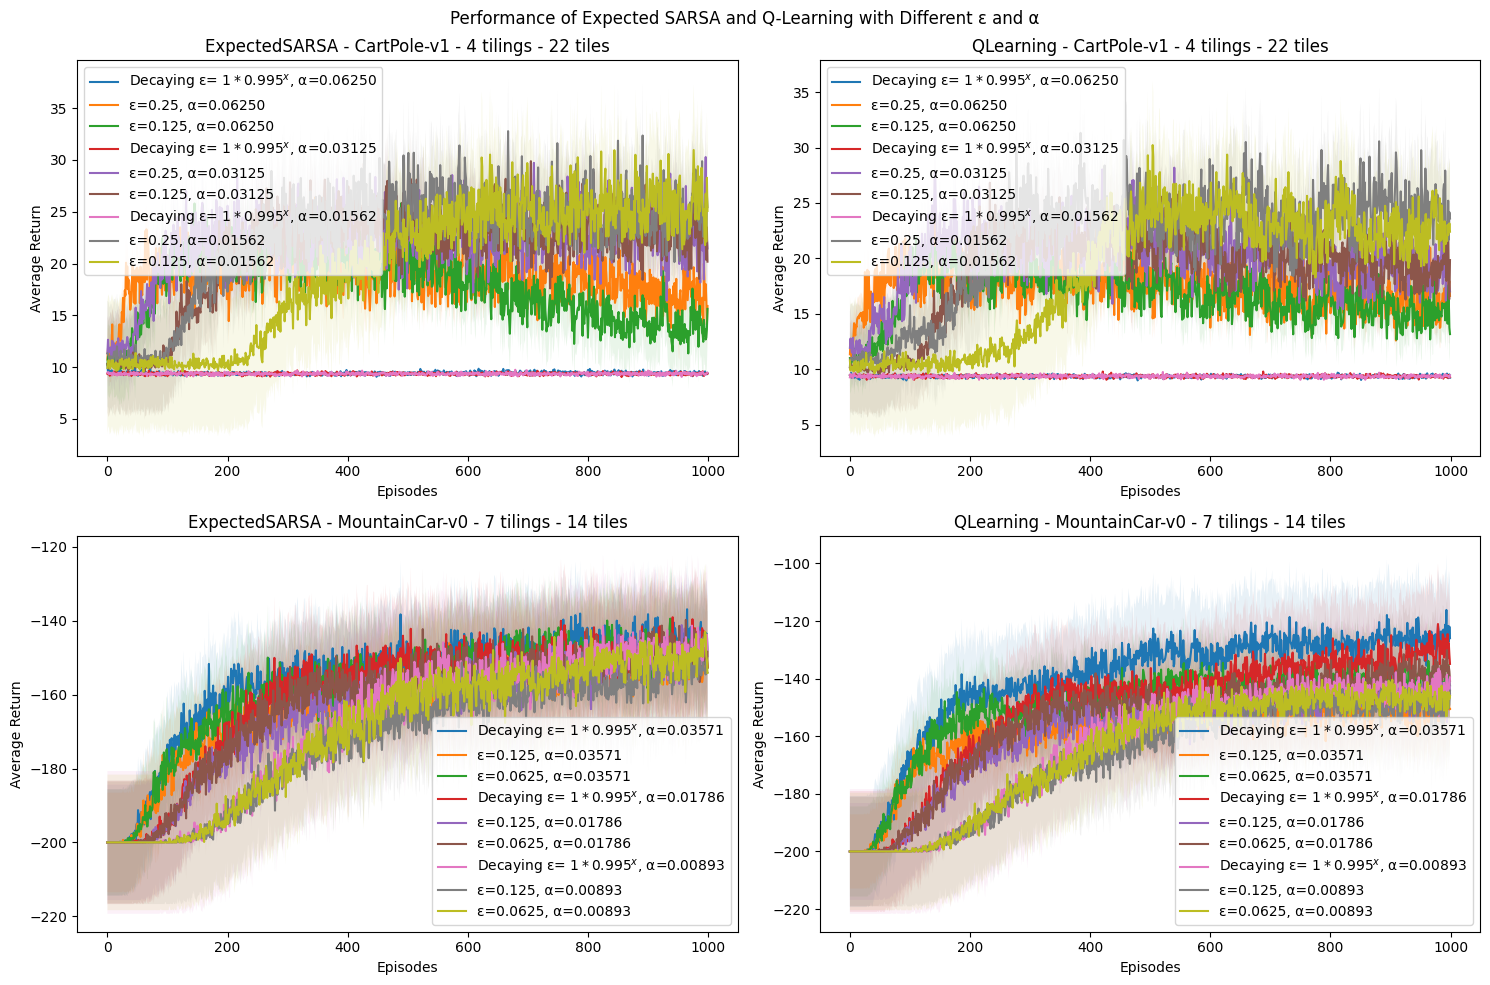
\includegraphics[scale=0.33]{q1.png}
    \caption{ExpectedSARSA and Q-Learning's Performances on CartPole-v1 and MountainCar-v0}
    \label{fig:q1}
\end{figure}

\subsection{Discussion}


\section{Policy Gradient Theorem}

\section{Policy-based methods with linear function approximation}

\subsection{Results}

\subsection{Discussion}

\newpage
\bibliography{ref}{}
\bibliographystyle{plain}
\end{document}
